\documentclass[conference]{IEEEtran}
% \IEEEoverridecommandlockouts   % uncomment only if \thanks is needed
\usepackage{cite}
\usepackage{amsmath,amssymb,amsfonts}
\usepackage{algorithmic}
\usepackage{graphicx}
\usepackage{textcomp}
\usepackage{xcolor}
\usepackage{url}
\interdisplaylinepenalty=2500

\begin{document}

\title{SNP-AV1: Stacked Neural Pruners for the AV1\\ Intra-Frame Partition Search}

\author{\IEEEauthorblockN{Pablo Rosa}
\IEEEauthorblockA{\textit{Video Technology Research Group (ViTech)} \\
\textit{Federal University of Pelotas} \\
Pelotas, Brazil \\
pablo.rosa@inf.ufpel.edu.br}
\and
\IEEEauthorblockN{Daniel Palomino}
\IEEEauthorblockA{\textit{Video Technology Research Group (ViTech)} \\
\textit{Federal University of Pelotas} \\
Pelotas, Brazil \\
dpalomino@inf.ufpel.edu.br}
\and
\IEEEauthorblockN{Marcelo Porto}
\IEEEauthorblockA{\textit{Video Technology Research Group (ViTech)} \\
\textit{Federal University of Pelotas} \\
Pelotas, Brazil \\
porto@inf.ufpel.edu.br}
\and
\IEEEauthorblockN{Luciano Agostini}
\IEEEauthorblockA{\textit{Video Technology Research Group (ViTech)} \\
\textit{Federal University of Pelotas} \\
Pelotas, Brazil \\
agostini@inf.ufpel.edu.br}
}

\maketitle

\begin{abstract}
The intra-frame coding of the AOMedia Video 1 (AV1) codec relies on a recursive
block partition search that evaluates ten candidate shapes at each node of the
partition tree. At the highest-quality configuration this search is
exhaustive by construction and dominates the intra-frame encoding time. This
paper presents the Stacked Neural Pruners for AV1 (SNP-AV1), a fast decision
algorithm for the intra-frame partition search applying two neural networks at
two distinct stages of a single node. The first reads thirty-six attributes of
causal context, whose extraction cost is negligible, and decides before any
rate-distortion evaluation how much of the subtree deserves to be opened. The
second adds the measured rate-distortion cost of the undivided candidate and
decides whether the AB and 4-way shapes, which take one third of the local search
time and which no earlier pruner targeted, are evaluated at all. The two are
stacked because the candidates they remove are disjoint. Experimental results
show that SNP-AV1 achieves an average time savings of 18.74\% with a Bjontegaard
delta bitrate (BD-BR) of 0.59\%, reaching 32.16\% and 1.42\% under a stronger
calibration, and the second pruner buys time about 3.4 times cheaper than
loosening the thresholds of the first. To the best of the authors' knowledge,
this is the first solution in the literature to prune the extended partitions of
the AV1 intra-frame partition search with a learned model.
\end{abstract}

\begin{IEEEkeywords}
Video coding, AV1, computational effort reduction, intra-frame block
partitioning, machine learning, neural networks.
\end{IEEEkeywords}

\section{Introduction}
\label{sec_intro}

Video is the dominant workload of the Internet, and the share of users watching
online video every month has kept growing over the last years \cite{statista}.
Alongside the standards defined by the international standardization bodies, such
as the High Efficiency Video Coding (HEVC) \cite{hevc} and the Versatile Video
Coding (VVC) \cite{vvc}, developed by the Motion Picture Expert Group (ISO/IEC
MPEG) and by the Video Coding Experts Group (ITU-T VCEG), the Alliance for Open
Media (AOMedia) maintains the AOMedia Video 1 (AV1) \cite{av1site}, which follows
the state-of-the-art flow of hybrid video encoders, splitting the process into
intra-frame prediction, inter-frame prediction, transforms, quantization, in-loop
filters and entropy coding, and introduced new techniques in each of these steps
\cite{han2021,chen2018}. This coding efficiency comes at the
price of computational effort: AV1 was shown to be superior to HEVC under certain
conditions \cite{grois2016}, but encoding videos of the same bitrate and
resolution took twice as long \cite{layek2017}, a problem aggravated during UHD
4K content processing.

One of the largest individual costs of AV1 intra-frame coding is the block
partitioning decision. Every superblock is submitted to a recursive search that,
at each node of the partition tree, evaluates the rate-distortion (RD) cost
\cite{sullivan1998} of ten candidate shapes and keeps the cheapest one,
descending recursively whenever the quad-tree split wins. The search is
exhaustive by construction, since the encoder can only determine the best shape
after evaluating the block under each candidate, and the reference software
libaom \cite{libaom} performs it in full at the highest-quality setting,
\texttt{cpu-used=0}.

There are a few works in the literature targeting the computational effort of
AV1, and none of them deals with this search. The works \cite{xu2020,xu2021,%
jeong2019} act on the intra prediction mode decision loop, while
\cite{correa2020,netto2022} are hardware solutions for the AV1 intra prediction,
whose target is the circuit and not the encoder search, and \cite{kim2019} uses
decision trees to determine whether all inter-prediction modes need to be
evaluated. Learning-based partitioning solutions do exist for VVC
\cite{saldanha2022,he2021,chen2019} and can be adapted to the AV1 coding tools,
but they were designed for the quad-tree with nested multi-type tree and
evaluated on another encoder. None of these papers allow a direct and fair
comparison, and none of them acts on the recursive partition search of the AV1
intra-frame coding.

This paper presents the Stacked Neural Pruners for AV1 (SNP-AV1), a fast decision
algorithm confined to the intra-frame partition search, which leaves every other
encoding stage untouched. The main strategy of this solution is to remove
candidates progressively, as stronger evidence becomes available: a first network
decides how much of the partition tree deserves to be opened, from causal context
whose extraction cost is negligible, and a second decides whether the most
expensive family of candidates is worth evaluating, from the rate-distortion
evidence the encoder has measured by then. The two are stacked because the sets
of candidates they remove are disjoint, which is the condition under which the
savings of two pruners accumulate instead of competing for the same time. Over
the eight UHD 4K video sequences of the Common Test Conditions (CTC) Class A1,
SNP-AV1 reaches an average time savings of 18.74\% with a Bj{\o}ntegaard delta
bitrate (BD-BR) of 0.586\%.

\section{Block Partitioning in AV1}
\label{sec_shapes}

The basic unit of the AV1 partitioning is the superblock, which has 128$\times$128
or 64$\times$64 pixels, and the structure that subdivides it is called partition
tree \cite{han2021}. AV1 allows ten partition types at each node \cite{chen2018},
which Fig.~\ref{fig_shapes} names and organizes into the four families used
throughout this paper: the two structural decisions, PARTITION\_NONE, hereafter
NONE, which codes the node undivided, and PARTITION\_SPLIT, the quad-tree split
into four square sub-blocks; the two rectangular shapes; the four asymmetric AB
shapes, each combining one rectangular half with two square sub-blocks; and the
two 4-way shapes, of 4:1 aspect ratio. The AB and the 4-way families are jointly
called the extended partitions.

\begin{figure}[!t]
  \centering
  % src/scripts/benchmark/plot_partition_shapes_fig1.py
  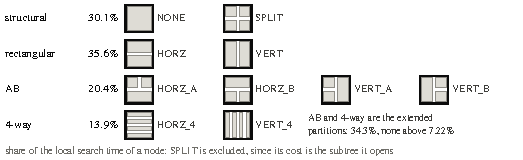
\includegraphics[width=\columnwidth]{fig1_partition_shapes}
  \caption{The ten partition shapes evaluated at a node, grouped into the four
  families used in this work and annotated with the share of local search time
  each family consumes.}
  \label{fig_shapes}
\end{figure}

The evaluation order inside a node is fixed and defines which information has
already been paid at each point of the flow: NONE, the quad-tree split, the
rectangular shapes and finally the extended partitions. A pruner acting before
the first evaluation is blind to any rate-distortion number, and one acting after
NONE has the measured rate, distortion and RD cost of the undivided candidate, at
the price of never saving the cost of producing them.

The cost distribution in Fig.~\ref{fig_shapes} was measured with the native
partition timing instrumentation of libaom over 875{,}317 decision nodes of the
4K videos described in Section \ref{sec_data}, at \texttt{cpu-used=0}, taking as
local work the sum of the nine non-recursive candidates of a node. It splits into
three blocks of comparable size: NONE takes 30.1\% of that time, the two
rectangular shapes take 35.6\% and the six extended ones take 34.3\%. No single
extended shape exceeds 7.22\%, which is why the weight of the family as a whole
went unnoticed, and the cost concentrates in the large nodes, reaching 50.0\% at
32$\times$32 and 51.0\% at 64$\times$64 pixels, which are the nodes a 4K frame
produces in abundance.

This work is focused on the acceleration of the recursive block partitioning
decision of the AV1 intra-frame coding. The other decisions taken inside a coding
block, such as the intra prediction modes, the transform type search and the
in-loop filtering, lie outside the partition search loop attacked here, as does
the inter-frame partition search, since the solution is trained and evaluated
exclusively under the All-Intra (AI) encoder configuration.

\section{Proposed SNP-AV1 Solution}
\label{sec_method}

The Stacked Neural Pruners for AV1 (SNP-AV1) is a fast decision algorithm
composed of two neural pruners inserted at two distinct stages of the search of a
node, as shown in Fig.~\ref{fig_snp}. The main strategy of this solution is to
consult each pruner at the earliest point of the flow at which the information it
needs has already been paid for.

\begin{figure}[!t]
  \centering
  % src/scripts/benchmark/plot_pruner_flowchart_fig2.py
  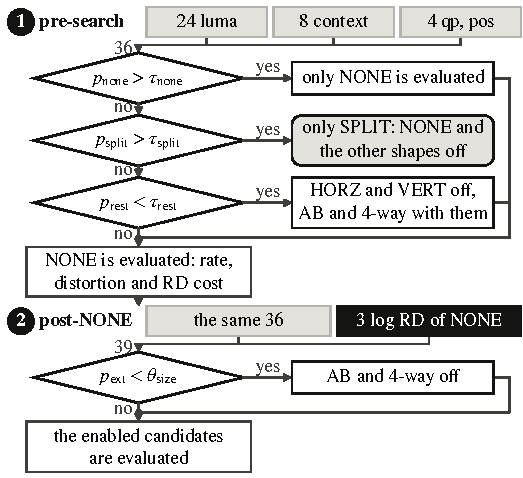
\includegraphics[width=\columnwidth]{fig2_insertion_points}
  \caption{Insertion points of the two pruners in the search of a node, and the
  cascade of conditions each of them applies.}
  \label{fig_snp}
\end{figure}

The two stages are complementary rather than competing. The first acts before any
rate-distortion evaluation, so a commitment removes every competing candidate of
the node and the whole subtree below it, including the evaluation of NONE at each
descendant; it pays for that reach by deciding blind to rate-distortion. The
second acts only on the nodes that survive the first and reads the measured RD
cost of NONE, over a narrower scope: the AB and 4-way candidates still standing.

The rule behind the pairing is that two pruners inserted in the same search
compete for the same saved time whenever they remove the same candidates, however
different the information each of them reads, and accumulate whenever the sets
they remove are disjoint. The first stage asks whether the node can be settled at
once, on the structural axis of NONE against the quad-tree split; the second asks
whether the extended partitions, the block of cost isolated in
Section~\ref{sec_shapes}, are worth evaluating. One limit follows from the same
rule, and Section~\ref{sec_results} measures it: a node the first stage has
committed never reaches the second, so the disjunction that makes the two
additive is a property of the operating point, and not of the pruners.

\subsection{Attribute Design}

The attribute vector of the first stage has thirty-six entries. Twenty-four are
luma descriptors of the node and of its hierarchical context, covering variance,
gradient energy and orientation, row and column profiles, edge strength and
density, and the contrast against the parent and the sibling sub-blocks. Eight
carry the causal partitioning neighborhood, that is, the availability of the
above and left neighbors, their decided widths and heights in log2 units and
their granularity and anisotropy; the last four carry the effective
dequantization step of the luma DC coefficient, the normalized position in the
frame and the node depth.

The criterion for inclusion was the cost of obtaining each attribute where the
pruner is consulted: the twelve neighborhood, quantization and position entries
are a free read of state the native search already maintains, and the luma
descriptors require only arithmetic linear in the area of the node. The second
stage reads these thirty-six plus the logarithm of the rate, of the distortion
and of the RD cost measured for NONE. Every luma sample is brought to the
eight-bit scale before any descriptor is computed, and the dequantization step
with it, so no attribute depends on the bit depth and the models trained on
eight-bit material are deployed unchanged on the ten-bit evaluation sequences.

\subsection{Dataset Construction}
\label{sec_data}

The reference software libaom v3.10.0 was instrumented under a compile-time guard
to record, at every node of the intra-frame partition search, the decision taken
by the encoder itself together with the luma samples, the causal context, the
quantization state, the position and the rate-distortion result of NONE. The
guard is necessary because a binary that writes to disk at every node cannot
measure wall-clock acceleration.

The dataset was built from the sixteen 4K sequences of the UVG dataset
\cite{uvg}, at 3840$\times$2160, 8-bit depth and 4:2:0 chroma subsampling, each
encoded at CQ 20, 32, 43 and 55 over five frames sampled uniformly along the
whole clip, since in AI coding consecutive frames are nearly identical. The
extraction ran entirely at \texttt{cpu-used=0}, because the label is only
faithful if it comes from a search that evaluated every candidate shape: an
extraction at \texttt{cpu-used=6} produced zero counts for the six extended
classes, exactly the ones the second stage must predict.

The resulting dataset contains 26.98 million samples, of which 10.07 million are
decision nodes of 16, 32 and 64 pixels; the rest are 8$\times$8 leaves whose
label is constant and which are left out of the modeling. It was partitioned by
sequence into ten training, three validation and three reserved test sequences,
frozen before any measurement, and the eight evaluation sequences belong to the
CTC Class A1 set, absent from the UVG corpus, so no sequence is reused across
training, testing and evaluation, which rules out data leakage.

\subsection{Network Architecture and Training}

Both stages use multilayer perceptrons, one per node size, trained independently
for the 16$\times$16, 32$\times$32 and 64$\times$64 levels; the 8$\times$8 level
is terminal and is not modeled. The topology is common to all six networks and
deliberately shallow: two hidden layers of 64 and 32 rectified units and a linear
output whose softmax gives three class probabilities in the first stage and two
in the second, for 27{,}759 parameters in total. They were trained in PyTorch
\cite{pytorch} with the AdamW optimizer \cite{adamw}, a learning rate of
$1 \times 10^{-3}$, a weight decay of $1 \times 10^{-4}$, batches of 4096 samples
and a fixed budget of 30 epochs, under hard-label cross entropy without class
weighting. The attributes are standardized during training and the
standardization is folded into the first linear layer at export time, so the
encoder feeds raw attributes and the models execute natively within the encoding
pipeline; this parity was verified over 192 random vectors, with a maximum
difference of $1.35 \times 10^{-7}$.

On the reserved sequences, and before any encoder integration, the expected
calibration error of the first stage is 0.0112 over 1{,}816{,}393 held-out
decision nodes, so reading its thresholds as confidence levels is verified rather
than assumed, and the three rate-distortion attributes raise the area under the
receiver operating characteristic curve of the second from 0.890 to 0.902, enough
to avoid half of the extended searches while losing 1.1\% of their true winners.

\subsection{Pruning Policies and Encoder Integration}

The first-stage pruner applies three actions in cascade, drawn in
Fig.~\ref{fig_snp}, on the probabilities $p_{\mathrm{none}}$,
$p_{\mathrm{split}}$ and $p_{\mathrm{rest}}$ of the undivided, split and
remaining classes. If $p_{\mathrm{none}} > \tau_{\mathrm{none}}$, the node is
decided as NONE and the whole subtree is cut, which is the primary lever of time
savings. Otherwise, if $p_{\mathrm{split}} > \tau_{\mathrm{split}}$, NONE is
skipped as well and the search recurses only into the four sub-blocks.
Otherwise, if $p_{\mathrm{rest}} < \tau_{\mathrm{rest}}$, the rectangular
candidates are disabled, and the extended ones with them by dependency;
otherwise the node proceeds to the full search. Two operating points were frozen
before the final campaign: the balanced one uses $\tau_{\mathrm{none}} = 0.95$,
$\tau_{\mathrm{split}} = 0.90$ and $\tau_{\mathrm{rest}} = 0.20$, the aggressive
one 0.60, 0.85 and 0.40.

The second-stage pruner marks the node to skip the extended partitions when
$p_{\mathrm{ext}}$, the estimated probability that an AB or a 4-way shape wins
the node, falls below a threshold $\theta$ kept per node size, leaving NONE, the
quad-tree split and the rectangular shapes untouched. The per-level threshold is
experimental, since the values that discard the same fraction of true winners
differ widely: calibrated on the reserved sequences to lose a tenth of the nodes
whose optimal shape is extended, the deployed values are 0.0910, 0.1031 and
0.0144 at the 16, 32 and 64-pixel levels, and a stronger calibration gives
0.1776, 0.1627 and 0.0321.

Both pruners were implemented in C inside libaom v3.10.0, each behind a
compile-time guard whose disabled build reproduces the reference bitstream byte
for byte, which is what allows the marginal contribution of the second to be
attributed to its decisions and not to a difference of build. The policy only
removes candidates and never forces an illegal one, so SNP-AV1 is fully compliant
with the AV1 specification and does not affect the bitstream syntax.

\section{Results and Comparisons}
\label{sec_results}

The developed solution was evaluated using the libaom v3.10.0 AV1 reference
software, following the AOM Common Test Conditions (CTC) \cite{ctc} and under the
AI encoder configuration. The eight 4K sequences of the CTC Class A1 test set,
named in Table~\ref{tab_seq}, are all at 3840$\times$2160, 10 bits and 4:2:0
\cite{xipha1}. The first 15 frames of each were encoded, as the CTC specifies for
the AI scenario, at CQ 20, 32, 43 and 55, against the unmodified libaom at
\texttt{cpu-used=0} as anchor. The BD-BR \cite{bjontegaard} is computed over the
luma peak signal-to-noise ratio, and all values reported here are positive, hence
coding efficiency losses. Writing $t_{\mathrm{cfg}}(s,q)$ and
$t_{\mathrm{anc}}(s,q)$ for the encoding times of the evaluated configuration and
of the anchor on sequence $s$ at quality point $q$, over the sequence set $S$ and
the quality set $Q$,

\begin{equation}
\mathrm{TS} = \frac{1}{|S|} \sum_{s \in S} \frac{1}{|Q|} \sum_{q \in Q}
\left( 1 - \frac{t_{\mathrm{cfg}}(s,q)}{t_{\mathrm{anc}}(s,q)} \right),
\label{eq_ts}
\end{equation}

reported as a percentage. All BD-BR and TS results come from this grid; the
shares in Fig.~\ref{fig_shapes} were measured on the UVG corpus of
Section~\ref{sec_data} instead. Every configuration was encoded once, and
repeating the anchor and the balanced first stage five times on Crosswalk gives a
standard deviation of 0.23 percentage points on TS, so a difference of time
savings below twice that value is not resolved. The BD-BR values carry no such
caveat, since the byte count and the luma PSNR are deterministic.

One scope decision governs the comparisons that follow. The anchor is the
exhaustive partition search itself, and no native speed preset is placed beside
SNP-AV1: a preset reconfigures dozens of heuristics spread over every coding
stage, whereas SNP-AV1 acts inside the partition search alone, so a side-by-side
reading would rank arrangements of different scope rather than partition-search
techniques.

Fig.~\ref{fig_space} places the six measured operating points of SNP-AV1 against
that anchor. The balanced calibration spans time savings of 17.72\% to 19.81\% at
a BD-BR of 0.568\% to 0.651\%, and the aggressive one 31.51\% to 32.16\% at
1.403\% to 1.420\%. Inside each family the three points differ only in how much
of the extended family the second pruner removes, and moving from one family to
the other is a matter of thresholds alone, without retraining and without
recompiling.

\begin{table}[!t]
\renewcommand{\arraystretch}{1.15}
\caption{Per-Sequence Results of the Two Deployed Operating Points Against the
libaom v3.10.0 Anchor at \upshape cpu-used=0}
\label{tab_seq}
\centering
\begin{tabular}{lcccc}
\hline
 & \multicolumn{2}{c}{\textbf{Balanced}} & \multicolumn{2}{c}{\textbf{Aggressive}} \\
\textbf{Sequence} & \textbf{BD-BR} & \textbf{TS} & \textbf{BD-BR} & \textbf{TS} \\
\hline
BoxingPractice & 0.662\% & 20.33\% & 1.560\% & 31.97\% \\
Crosswalk & 0.534\% & 20.53\% & 1.145\% & 35.08\% \\
FoodMarket2 & 0.609\% & 14.14\% & 1.386\% & 26.74\% \\
Neon1224 & 0.685\% & 22.00\% & 1.427\% & 33.05\% \\
NocturneDance & 0.168\% & 13.78\% & 1.209\% & 30.79\% \\
PierSeaSide & 0.458\% & 17.47\% & 1.403\% & 26.03\% \\
Tango & 1.139\% & 22.89\% & 2.206\% & 38.80\% \\
TimeLapse & 0.433\% & 18.78\% & 0.934\% & 31.00\% \\
\hline
\textbf{Average} & \textbf{0.586\%} & \textbf{18.74\%} & \textbf{1.409\%} & \textbf{31.68\%} \\
\hline
\end{tabular}
\end{table}

The second stage is measured marginally, because it acts only on the residue of
nodes the first stage did not commit. Over the balanced base it contributes 1.02
percentage points of time savings, about 4.4 times the measured standard
deviation, for 0.018 percentage points of BD-BR. That is a price of 0.018 point
of coding efficiency per point of time bought, against the 0.061 charged by the
only alternative the deployed solution leaves to its user, which is loosening the
thresholds of the first stage: the second pruner is about 3.4 times cheaper, and
Fig.~\ref{fig_space}(a) shows the two prices as the two slopes that leave the
same operating point. Its stronger calibration costs 0.040 over the
same base, still below the price of the threshold knob, which is why the milder
one is deployed. Sequence by sequence, at time savings matched by interpolating
the first-stage thresholds, the stacked point is the better of the two in six of
the eight sequences, two of them by strict Pareto dominance, and it loses only in
Crosswalk and Neon1224, the two sequences in which the extended axis is barely
exercised and the second pruner has almost nothing to remove.

\begin{figure}[!t]
  \centering
  % src/scripts/benchmark/plot_operating_space_fig3.py
  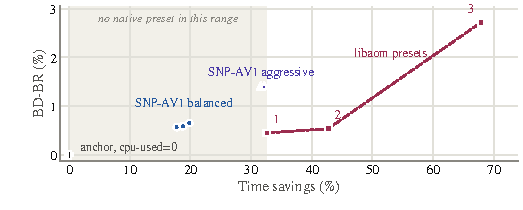
\includegraphics[width=\columnwidth]{fig3_operating_space}
  \caption{Operating space of SNP-AV1 against the libaom v3.10.0 anchor at
  \texttt{cpu-used=0}, over the CTC Class A1 4K sequences: (a) balanced and
  (b) aggressive calibration, each on its own axes. Inside each panel the three
  points differ only in the strength of the second pruner, and the dashed line is
  the threshold knob of the first stage.}
  \label{fig_space}
\end{figure}

This additivity is a property of the operating point, and not of the pruner. Over
the aggressive base the same second stage adds 0.17 percentage points, below the
resolution of the arrangement and above it in one sequence out of eight instead
of six. With the undivided threshold loosened to 0.60, the first stage commits
the nodes so early that they seldom reach the point at which the extended
partitions would be decided, and the two pruners fall back to disputing the same
residue. Fig.~\ref{fig_space}(b) shows what is left of the second stage there:
the three points cover 0.65 percentage points of time savings, and the step the
deployed calibration adds is 0.17 of them.

Table~\ref{tab_seq} opens the two deployed points per sequence, and what it
exposes is content dispersion, not a swept range. Read as time bought per point
of coding efficiency ceded, the median of the eight sequences is 35 points of
time savings per point of BD-BR at the balanced point and 22 at the aggressive
one, the same rising price the aggregate already showed. Tango is the least
favorable sequence under both calibrations, and the two columns move together
across the set: the sequences in which the first stage commits the most nodes are
also the ones in which committing costs the most.

The overhead is reported rather than omitted: the complete path of SNP-AV1,
attribute extraction and inference together, stays below one third of one percent
of the encoding time, so the time savings come from the pruning decisions and not
from the lightness of each inference.

\section{Conclusions}

This paper presented SNP-AV1, a machine-learning solution that stacks two neural
pruners at two distinct stages of the AV1 intra-frame partition search, reaching
an average time savings of 18.74\% with a BD-BR of 0.59\%, and 32.16\% with
1.42\% under a stronger calibration. The first pruner decides how much of the
subtree is opened before any rate-distortion cost is paid, and the second whether
the extended partitions, one third of the local search time, are worth
evaluating; the two are stacked because the candidates they remove are disjoint.
Both were implemented in C inside libaom v3.10.0 and evaluated on the eight 4K
sequences of the CTC Class A1 under the AI configuration, against the exhaustive
search as anchor. Measured marginally over the first, the second pruner adds 1.02
percentage points of time savings for 0.018 of BD-BR, about 3.4 times cheaper
than buying the same time from the thresholds of the first stage, and it is the
better of the two in six of the eight sequences; the advantage collapses on the
aggressive base, where the first stage commits the nodes before the second is
consulted. Besides, to the best of the authors' knowledge, this is the first
solution in the literature to prune the extended partitions of the AV1
intra-frame partition search with a learned model.

\section*{Acknowledgment}

This study was financed in part by the Coordena\c{c}\~ao de Aperfei\c{c}oamento de
Pessoal de N\'ivel Superior -- Brasil (CAPES) -- Finance Code 001, and also by the
Brazilian research support agencies CNPq and FAPERGS.

% \IEEEtriggeratref{n}  % set only when the last page needs balancing
\begin{thebibliography}{00}

\bibitem{statista} Statista. (2025). \emph{Share of Internet Users Watching Online Videos Every Month From 1st Quarter 2022 to 3rd Quarter 2024}. [Online]. Available: \url{https://www.statista.com/statistics/1489445/online-video-viewers-worldwide-quarterly/}

\bibitem{hevc} ITU-T. (2013). \emph{H.265: High Efficiency Video Coding}. [Online]. Available: \url{https://www.itu.int/rec/t-rec-h.265}

\bibitem{vvc} ITU-T. (2020). \emph{H.266: Versatile Video Coding}. [Online]. Available: \url{https://www.itu.int/rec/t-rec-h.266}

\bibitem{av1site} Alliance for Open Media. (2019). \emph{AV1 Video Codec}. [Online]. Available: \url{https://aomedia.org/av1}

\bibitem{han2021} J. Han \emph{et al.}, ``A technical overview of AV1,'' \emph{Proc. IEEE}, vol. 109, no. 9, pp. 1435--1462, Sep. 2021.

\bibitem{chen2018} Y. Chen \emph{et al.}, ``An overview of core coding tools in the AV1 video codec,'' in \emph{Proc. Picture Coding Symp. (PCS)}, Jun. 2018, pp. 41--45.

\bibitem{grois2016} D. Grois, T. Nguyen, and D. Marpe, ``Coding efficiency comparison of AV1/VP9, H.265/MPEG-HEVC, and H.264/MPEG-AVC encoders,'' in \emph{Proc. Picture Coding Symp. (PCS)}, Dec. 2016, pp. 1--5.

\bibitem{layek2017} M. A. Layek \emph{et al.}, ``Performance analysis of H.264, H.265, VP9 and AV1 video encoders,'' in \emph{Proc. 19th Asia-Pacific Netw. Oper. Manage. Symp. (APNOMS)}, Sep. 2017, pp. 322--325.

\bibitem{sullivan1998} G. J. Sullivan and T. Wiegand, ``Rate-distortion optimization for video compression,'' \emph{IEEE Signal Process. Mag.}, vol. 15, no. 6, pp. 74--90, Nov. 1998.

\bibitem{libaom} Alliance for Open Media. \emph{AV1 Codec Library}, v3.10.0. [Online]. Available: \url{https://aomedia.googlesource.com/aom}

\bibitem{xu2020} M. Xu and B. Jeon, ``Selection of intra prediction tools for fast AV1 encoding,'' in \emph{Proc. IEEE Int. Symp. Broadband Multimedia Syst. Broadcast. (BMSB)}, Oct. 2020, pp. 1--4.

\bibitem{xu2021} M. Xu and B. Jeon, ``User-priority based AV1 coding tool selection,'' \emph{IEEE Trans. Broadcast.}, vol. 67, no. 3, pp. 736--745, Sep. 2021.

\bibitem{jeong2019} J. Jeong, G. Gankhuyag, and Y.-H. Kim, ``A fast intra mode decision based on accuracy of rate distortion model for AV1 intra encoding,'' in \emph{Proc. 34th Int. Tech. Conf. Circuits/Syst., Comput. Commun. (ITC-CSCC)}, Jun. 2019, pp. 1--3.

\bibitem{correa2020} M. Corr\^ea, B. Zatt, D. Palomino, G. Corr\^ea, and L. Agostini, ``A high-throughput hardware architecture for AV1 non-directional intra modes,'' \emph{IEEE Trans. Circuits Syst. I, Reg. Papers}, vol. 67, no. 5, pp. 1481--1494, May 2020.

\bibitem{netto2022} L. Netto, M. Corr\^ea, D. Palomino, L. Agostini, and G. Corr\^ea, ``Power-quality configurable hardware design for AV1 directional intra-frame prediction,'' \emph{IEEE Design Test}, vol. 39, no. 2, pp. 38--45, Apr. 2022.

\bibitem{kim2019} J. Kim, S. Blasi, A. S. Dias, M. Mrak, and E. Izquierdo, ``Fast inter-prediction based on decision trees for AV1 encoding,'' in \emph{Proc. IEEE Int. Conf. Acoust., Speech Signal Process. (ICASSP)}, May 2019, pp. 1627--1631.

\bibitem{saldanha2022} M. Saldanha, G. Sanchez, C. Marcon, and L. Agostini, ``Configurable fast block partitioning for VVC intra coding using light gradient boosting machine,'' \emph{IEEE Trans. Circuits Syst. Video Technol.}, vol. 32, no. 6, pp. 3947--3960, Jun. 2022.

\bibitem{he2021} Q. He, W. Wu, L. Luo, C. Zhu, and H. Guo, ``Random forest based fast CU partition for VVC intra coding,'' in \emph{Proc. IEEE Int. Symp. Broadband Multimedia Syst. Broadcast. (BMSB)}, Aug. 2021, pp. 1--4.

\bibitem{chen2019} J. Chen, H. Sun, J. Katto, X. Zeng, and Y. Fan, ``Fast QTMT partition decision algorithm in VVC intra coding based on variance and gradient,'' in \emph{Proc. IEEE Vis. Commun. Image Process. (VCIP)}, Dec. 2019, pp. 1--4.

\bibitem{uvg} A. Mercat, M. Viitanen, and J. Vanne, ``UVG dataset: 50/120fps 4K sequences for video codec analysis and development,'' in \emph{Proc. 11th ACM Multimedia Syst. Conf. (MMSys)}, Jun. 2020, pp. 297--302.

\bibitem{pytorch} A. Paszke \emph{et al.}, ``PyTorch: An imperative style, high-performance deep learning library,'' in \emph{Proc. Adv. Neural Inf. Process. Syst. (NeurIPS)}, Dec. 2019, pp. 8024--8035.

\bibitem{adamw} I. Loshchilov and F. Hutter, ``Decoupled weight decay regularization,'' in \emph{Proc. Int. Conf. Learn. Represent. (ICLR)}, May 2019, pp. 1--18.

\bibitem{ctc} X. Zhao \emph{et al.}, ``AOM common test conditions v9.0,'' Alliance for Open Media, Codec Working Group, doc. CWG-G082, Mar. 2026.

\bibitem{xipha1} Xiph.Org Foundation. \emph{AOM CTC Test Set, Class A1 (4K)}. [Online]. Available: \url{https://media.xiph.org/video/aomctc/test_set/a1_4k/}

\bibitem{bjontegaard} G. Bj{\o}ntegaard, ``Calculation of average PSNR differences between RD-curves,'' Video Coding Experts Group (VCEG), doc. VCEG-M33, Mar. 2001.

\end{thebibliography}

\end{document}
